 %%
%% Beginning of file 'sample61.tex'
%%
%% Modified 2016 September
%%
%% This is a sample manuscript marked up using the
%% AASTeX v6.1 LaTeX 2e macros.
%%
%% AASTeX is now based on Alexey Vikhlinin's emulateapj.cls 
%% (Copyright 2000-2015).  See the classfile for details.

%% AASTeX requires revtex4-1.cls (http://publish.aps.org/revtex4/) and
%% other external packages (latexsym, graphicx, amssymb, longtable, and epsf).
%% All of these external packages should already be present in the modern TeX 
%% distributions.  If not they can also be obtained at www.ctan.org.

%% The first piece of markup in an AASTeX v6.x document is the \documentclass
%% command. LaTeX will ignore any data that comes before this command. The 
%% documentclass can take an optional argument to modify the output style.
%% The command below calls the preprint style  which will produce a tightly 
%% typeset, one-column, single-spaced document.  It is the default and thus
%% does not need to be explicitly stated.
%%
%%
%% using aastex version 6.1
\documentclass[twocolumn]{aastex61}

%% The default is a single spaced, 10 point font, single spaced article.
%% There are 5 other style options available via an optional argument. They
%% can be envoked like this:
%%
%% \documentclass[argument]{aastex61}
%% 
%% where the arguement options are:
%%
%%  twocolumn   : two text columns, 10 point font, single spaced article.
%%                This is the most compact and represent the final published
%%                derived PDF copy of the accepted manuscript from the publisher
%%  manuscript  : one text column, 12 point font, double spaced article.
%%  preprint    : one text column, 12 point font, single spaced article.  
%%  preprint2   : two text columns, 12 point font, single spaced article.
%%  modern      : a stylish, single text column, 12 point font, article with
%% 		  wider left and right margins. This uses the Daniel
%% 		  Foreman-Mackey and David Hogg design.
%%
%% Note that you can submit to the AAS Journals in any of these 6 styles.
%%
%% There are other optional arguments one can envoke to allow other stylistic
%% actions. The available options are:
%%
%%  astrosymb    : Loads Astrosymb font and define \astrocommands. 
%%  tighten      : Makes baselineskip slightly smaller, only works with 
%%                 the twocolumn substyle.
%%  times        : uses times font instead of the default
%%  linenumbers  : turn on lineno package.
%%  trackchanges : required to see the revision mark up and print its output
%%  longauthor   : Do not use the more compressed footnote style (default) for 
%%                 the author/collaboration/affiliations. Instead print all
%%                 affiliation information after each name. Creates a much
%%                 long author list but may be desirable for short author papers
%%
%% these can be used in any combination, e.g.
%%
%% \documentclass[twocolumn,linenumbers,trackchanges]{aastex61}

%% AASTeX v6.* now includes \hyperref support. While we have built in specific
%% defaults into the classfile you can manually override them with the
%% \hypersetup command. For example,
%%
%%\hypersetup{linkcolor=red,citecolor=green,filecolor=cyan,urlcolor=magenta}
%%
%% will change the color of the internal links to red, the links to the
%% bibliography to green, the file links to cyan, and the external links to
%% magenta. Additional information on \hyperref options can be found here:
%% https://www.tug.org/applications/hyperref/manual.html#x1-40003

%% If you want to create your own macros, you can do so
%% using \newcommand. Your macros should appear before
%% the \begin{document} command.
%%
\newcommand{\vdag}{(v)^\dagger}
\newcommand\aastex{AAS\TeX}
\newcommand\latex{La\TeX}
%\newcommand{\dom}[1]{{\bf [[#1]]}} 
\newcommand{\dom}[1]{{#1}} 
%% Reintroduced the \received and \accepted commands from AASTeX v5.2
%\received{July 1, 2016}
%\revised{September 27, 2016}
%\accepted{\today}
%% Command to document which AAS Journal the manuscript was submitted to.
%% Adds "Submitted to " the arguement.
\submitjournal{ApJL}

%% Mark up commands to limit the number of authors on the front page.
%% Note that in AASTeX v6.1 a \collaboration call (see below) counts as
%% an author in this case.
%
%\AuthorCollaborationLimit=3
%
%% Will only show Schwarz, Muench and "the AAS Journals Data Scientist 
%% collaboration" on the front page of this example manuscript.
%%
%% Note that all of the author will be shown in the published article.
%% This feature is meant to be used prior to acceptance to make the
%% front end of a long author article more manageable. Please do not use
%% this functionality for manuscripts with less than 20 authors. Conversely,
%% please do use this when the number of authors exceeds 40.
%%
%% Use \allauthors at the manuscript end to show the full author list.
%% This command should only be used with \AuthorCollaborationLimit is used.

%% The following command can be used to set the latex table counters.  It
%% is needed in this document because it uses a mix of latex tabular and
%% AASTeX deluxetables.  In general it should not be needed.
%\setcounter{table}{1}

%%%%%%%%%%%%%%%%%%%%%%%%%%%%%%%%%%%%%%%%%%%%%%%%%%%%%%%%%%%%%%%%%%%%%%%%%%%%%%%%
%%
%% The following section outlines numerous optional output that
%% can be displayed in the front matter or as running meta-data.
%%
%% If you wish, you may supply running head information, although
%% this information may be modified by the editorial offices.
\shorttitle{Reionization of z=0 halos in Coda I-AMR}
\shortauthors{Aubert et al.}
%%
%% You can add a light gray and diagonal water-mark to the first page 
%% with this command:
% \watermark{text}
%% where "text", e.g. DRAFT, is the text to appear.  If the text is 
%% long you can control the water-mark size with:
%  \setwatermarkfontsize{dimension}
%% where dimension is any recognized LaTeX dimension, e.g. pt, in, etc.
%%
%%%%%%%%%%%%%%%%%%%%%%%%%%%%%%%%%%%%%%%%%%%%%%%%%%%%%%%%%%%%%%%%%%%%%%%%%%%%%%%%

%% This is the end of the preamble.  Indicate the beginning of the
%% manuscript itself with \begin{document}.

\begin{document}

%\title{The Reionization epoch of z=0 halos}
%\title{Connecting the Reionization history of galaxies to their z=0 properties}
\title{Relating the reionization times of galaxies to their present halo masses}


%% LaTeX will automatically break titles if they run longer than
%% one line. However, you may use \\ to force a line break if
%% you desire. In v6.1 you can include a footnote in the title.

%% A significant change from earlier AASTEX versions is in the structure for 
%% calling author and affilations. The change was necessary to implement 
%% autoindexing of affilations which prior was a manual process that could 
%% easily be tedious in large author manuscripts.
%%
%% The \author command is the same as before except it now takes an optional
%% arguement which is the 16 digit ORCID. The syntax is:
%% \author[xxxx-xxxx-xxxx-xxxx]{Author Name}
%%
%% This will hyperlink the author name to the author's ORCID page. Note that
%% during compilation, LaTeX will do some limited checking of the format of
%% the ID to make sure it is valid.
%%
%% Use \affiliation for affiliation information. The old \affil is now aliased
%% to \affiliation. AASTeX v6.1 will automatically index these in the header.
%% When a duplicate is found its index will be the same as its previous entry.
%%
%% Note that \altaffilmark and \altaffiltext have been removed and thus 
%% can not be used to document secondary affiliations. If they are used latex
%% will issue a specific error message and quit. Please use multiple 
%% \affiliation calls for to document more than one affiliation.
%%
%% The new \altaffiliation can be used to indicate some secondary information
%% such as fellowships. This command produces a non-numeric footnote that is
%% set away from the numeric \affiliation footnotes.  NOTE that if an
%% \altaffiliation command is used it must come BEFORE the \affiliation call,
%% right after the \author command, in order to place the footnotes in
%% the proper location.
%%
%% Use \email to set provide email addresses. Each \email will appear on its
%% own line so you can put multiple email address in one \email call. A new
%% \correspondingauthor command is available in V6.1 to identify the
%% corresponding author of the manuscript. It is the author's responsibility
%% to make sure this name is also in the author list.
%%
%% While authors can be grouped inside the same \author and \affiliation
%% commands it is better to have a single author for each. This allows for
%% one to exploit all the new benefits and should make book-keeping easier.
%%
%% If done correctly the peer review system will be able to
%% automatically put the author and affiliation information from the manuscript
%% and save the corresponding author the trouble of entering it by hand.

\correspondingauthor{Dominique Aubert}
\email{dominique.aubert@astro.unistra.fr}

\author{Dominique Aubert}
\affil{Observatoire Astronomique de Strasbourg \\
11 rue de l'Universite \\
67000, Strasbourg, France}

\author{Pierre Ocvirk}
\affil{Observatoire Astronomique de Strasbourg \\
11 rue de l'Universite \\
67000, Strasbourg, France}

\author{Nicolas Deparis}
\affil{Observatoire Astronomique de Strasbourg \\
11 rue de l'Universite \\
67000, Strasbourg, France}

\author{INCITE}
\affil{Observatoire Astronomique de Strasbourg \\
11 rue de l'Universite \\
67000, Strasbourg, France}

\author{CLUES}
\affil{Observatoire Astronomique de Strasbourg \\
11 rue de l'Universite \\
67000, Strasbourg, France}

%% Note that the \and command from previous versions of AASTeX is now
%% depreciated in this version as it is no longer necessary. AASTeX 
%% automatically takes care of all commas and "and"s between authors names.

%% AASTeX 6.1 has the new \collaboration and \nocollaboration commands to
%% provide the collaboration status of a group of authors. These commands 
%% can be used either before or after the list of corresponding authors. The
%% argument for \collaboration is the collaboration identifier. Authors are
%% encouraged to surround collaboration identifiers with ()s. The 
%% \nocollaboration command takes no argument and exists to indicate that
%% the nearby authors are not part of surrounding collaborations.

%% Mark off the abstract in the ``abstract'' environment. 
\begin{abstract}
The Reionization as experienced by galaxies is a diverse and heterogeneous process. We probe this diversity by presenting predictions of the Reionization times of z=0 galaxies made using simulations. The  $z>6$  epoch is described using the CODA~I-AMR radiative hydrodynamics simulation produced with the EMMA code.
%that models self-consistently the evolution of the gas ionisation state until the end of the first billion years of the Universe. This simulation has been 
%produced with the AMR code EMMA %and deployed on 32768 CPU cores and 4096 GPUs on Titan. 
High-redshift predictions are projected 13 billions years later using a pure dark matter Gadget simulation with the same set of CLUES initial conditions that include a Local Group analog. In both cases the $(64 \mathrm{Mpc/h})^3$ volume is sampled with  
%$2048^3\sim 8\times 10^9$ 
8 billions initial resolution elements,  allowing to probe halos in the $10^8-10^{13} M_\odot$ range. 

We find that current galaxies with $M_{z=0}>10^{11} M_\odot$ were reionized up to $\sim 500$ millions years earlier than the Universe as a whole.
%\since the progenitors of these objects form in the high peaks of the density field
%resulting from these objects being the hosts of the first sources. 
The scatter in Reionization times can be quite significant and Milky-Way like galaxies can have $z>6$ progenitors reionized as early as z=15 and as late as z=8. Less massive objects ($<10^{11} M_\odot$) are reionized at the same time as the overall volume or even later : this lag can be attributed to dark objects that require external radiation to complete their reionization. Measures of the reionization durations within halos show that the time required to reionize galaxies can be as large as the halo-to-halo fluctuation of reionization times. 

Finally, we find that Local Group was not influenced by an external sweeping ionization front. The Milky Way and M31 analogs of our simulation reionized respectively at z=9.8 and z=11, without influencing each other.


\end{abstract}

%% Keywords should appear after the \end{abstract} command. 
%% See the online documentation for the full list of available subject
%% keywords and the rules for their use.
\keywords{dark ages, reionization, first stars --- galaxies: high-redshift --- methods: numerical}

%% From the front matter, we move on to the body of the paper.
%% Sections are demarcated by \section and \subsection, respectively.
%% Observe the use of the LaTeX \label
%% command after the \subsection to give a symbolic KEY to the
%% subsection for cross-referencing in a \ref command.
%% You can use LaTeX's \ref and \label commands to keep track of
%% cross-references to sections, equations, tables, and figures.
%% That way, if you change the order of any elements, LaTeX will
%% automatically renumber them.

%% We recommend that authors also use the natbib \citep
%% and \citet commands to identify citations.  The citations are
%% tied to the reference list via symbolic KEYs. The KEY corresponds
%% to the KEY in the \bibitem in the reference list below. 

\section{Introduction}
The emergence of a UV background during the Reionization sets the thermal and ionisation state of the intergalactic medium. It can also suppress star formation in the progenitors of galaxies through photo-heating especially for low-mass objects below $10^9 M_\odot$. Accordingly, reconstructed star formation histories of the faintest dwarf galaxies indicate that the Reionization slowed down the build up of their stellar populations (see e.g. \citet{BROWN14}). Likewise recent radiative hydrodynamics simulations were able to reproduce this suppression in large high resolution simulations \citep{OCV16}. 

However, the Reionization is not a uniform and instantaneous process: the structure of the density field translate into an heterogeneous distribution of radiation sources and absorbers. Different patches and objects in the Universe do not reionize at the same time, but have widely ranging reionization redshifts. 
%For instance, Ly-$\alpha$ forest data suggest that the spatial fluctuations of the UV field remain important even after the overlap, possibly originating in the density field (e.g. \citet{DAV16}), temperature fluctuations (e.g. \citet{ALO15}) or the presence of bright UV sources (e.g. \citet{CHA15}).

The timing of the Reionization can have an impact on e.g. the satellite populations of z=0 galaxies (see e.g. \citet{KOP9,BUS10,OCV11,ILI11,OCV14,GIL15})
%Koposov et al. 2009; Busha et al. 2010, Ocvirk \& Aubert, 2011, Iliev et al. 2011, Ocvirk et al. 2014, Gillet et al. 2015) 
and the assumption on extended or instantaneous reionizations has a dramatic impact on the stellar populations of satellite galaxies. In a global context where the exact contribution of small galaxies to the Reionization is debated (see e.g. \citet{BOU14,FIN15}), all these aspects push for an improved description of the transition as seen from the high-z galaxies. 

In this letter, we want to determine the timings of the Reionization as experienced by today's galaxies and probe the heterogeneity of process. The main challenge is to connect contemporary objects to the Epoch of Reionization (EoR) : 13 billions years separate the Reionization from today and given the variety of build-up histories, it's not an easy task to determine the reionization context of a $z\ll6$ galaxy. To assess these questions, we combine for the first time a large scale dark-matter-only CLUES simulation at z=0 with a state-of-the-art AMR radiative hydrodynamics simulation of the EoR that self-consistently provides the reionization past of today galaxies, the CODA~I -AMR simulation. Because they share the same set of initial conditions (IC), these two simulations can be connected and predictions on the time and durations of the Reionization of z=0 galaxies can be made. Furthermore the ICs were constrained to include analogs of the Local Group (LG) in a realistic large-scale environment and allow us to assess how representative is the LG, arguably the best place to assess the past of small and old galaxies.  


%In the current letter, we explore the timings of the Reionization of $z = 0$ galaxies using a EMMA radiative hydrodynamics simulation of the Reionization \citep{AUB15} and extrapolating $z>6$ properties to $z=0$ using a pure DM Gadget simulation that shares the same initial conditions. We focus on the time and duration of the Reionization and we investigate briefly the impact of cosmic variance. 

The work presented here follow the lines of previous studies made by e.g. \citet{WEI07} or \citet{DIX17} who used radiative transfer post-processing of pre-existing simulations. It also complements \citet{ALV9} and \citet{LI14} who focused on scales and masses relevant for massive galaxies or clusters, using a semi-numerical methodology: thanks to the scales explored here ($64 h^{-1}$ Mpc box size sampled at a kpc resolution) we focus on smaller objects with masses between $10^8 M_\odot$ and $10^{13} M_\odot$. 
% and our methodology is entirely based on simulations. 
Our methodology is also similar to \citet{OCV14} on the LG Reionization. However, the current letter reassess this work by including the LG environment and by comparing it to the full population of galaxies. On a broader perspective, this work is also intended to introduce the CODA I-AMR simulation and presents the possibilities opened to investigate the EoR for galaxies in general and the LG in particular.


We first present our set of simulations and the analysis performed. We then describe the times and duration of reionizations for our simulated population of galaxies before discussing the case of the LG. Future investigations routes are then presented.

\section{Methods}

\subsection{Initial Conditions}
The initial conditions were created by the CLUES collaboration and assume a WMAP 5 cosmology ($\Omega_m=0.279, \Omega_v=0.721, H_0=70$ km/s/Mpc, \citet{HIN9}). They cover a $64$ Mpc/h comoving volume with a $2048^3$ grid cells and particles.  The initial phases were chosen to produce an analog of the Local Universe at z=0 (see \citet{GOT10},\citet{ILI11}) providing a Milky Way (MW)- M31 pair with the right mass range and separation in the proper large scale environment. These choices were motivated by future comparisons with the CODA I simulation \citep{OCV16}.

\subsection{Simulations}
The $z>6$ predictions of this project were produced by the AMR simulation code EMMA \citep{AUB15}. It tracks the coupled collisionless dynamics, hydrodynamics and radiative transfer and includes standard sub-grid models for star formation and supernovae feedback (\citet{DEP17}, in prep.). 

Space is sampled on a $2048^3$  grid that gets refined if it contains more than 8 DM particles. The grid is prevented to refine to physical resolutions smaller than 500 pc, corresponding to 3 additional levels of refinement by z=6 : the actual number of cells is then multiplied by 2.1, i.e. 18 billions cells. 

Star formation is triggered if the gas overdensity in a cell is greater than 50, ensuring that the first stellar particle appears at $z\sim 18$: once enabled, the star formation proceeds according to a Schmidt-Kenicutt Law with an efficiency of $1\%$ (see \citet{DEP17} in prep.). The stellar particles mass is  $7\times 10^4 M_\odot$. They produce ionizing photons according to a Starburst 99 population model \citep{LEI99} with a Top-Heavy IMF and 0.05 $Z_\odot$ metallicity : the corresponding emissivity is $1.5\times 10^{17}$ ionising photons/sec/stellar kg for $3\times 10^6$ years followed by an exponential decrease. Furthermore, an in-situ $20\%$ escape fraction is applied to compute the actual number of photons released in a simulation cell: it ensures a complete reionization at $z\sim 6$.  \dom{Radiation is propagated using the M1 radiative transfer method with a reduced speed of light $c_\mathrm{sim}=0.1$}. Mechanical feedback is enabled and a typical energy of $9.8\times 10^{11}$ J/stellar kg is released in the surrounding gas after $15\times 10^6$ years: 1/3 via thermal energy, 2/3 via kinetic winds. At z=6, $120\times 10^6$ stellar particles are present.

The CODA I-AMR simulation required 32768 CPUs and 4096 graphics devices (GPUs) on the TITAN (ORNL/DOE) supercomputer. The EMMA code is partially ported on GPU, accelerating the hydrodynamics and the radiative transfer: these modules are respectively 25 and 15 times faster on GPU than a single CPU core. Provided that each GPU is shared by 8 cores and that a substantial part of EMMA is exclusively managed by CPUs, the addition of 4096 GPUs to the 32768 cores leads to an 1.5 acceleration factor. 

%Finally, this simulation results from the conversion of a qualification run into a production one : it used a reduced speed of light ($c_\mathrm{sim}=0.1c$) that has been kept for the final run.

The CODA I-AMR simulation stopped at $z=6$: it presents a reionization epoch consistent with CMB constraints \citep{PLA15} but with a residual neutral fraction at lower levels than expected from quasars data (\citet{FAN6}, see Fig. \ref{fig:globpro}). The average star formation history is consistent with formation models obtained from the evolution of the high-z UV luminosity function \citep{BOU14,FIN15}.  

\begin{figure}[ht!]
%\plotone{img/x_sfr_tau.png}
\includegraphics[height=1.10\columnwidth, width=0.94\columnwidth]{img/x_sfr_tau.pdf}
\caption{The global average properties of the simulations. From top to bottom : the volume averaged ionization/neutral fraction history, the cosmic star formation rate and the CMB thomson scattering optical depth.}
\label{fig:globpro}
\end{figure}




%\subsection{z=0 Pure dark matter predictions}

The properties of z=0 halos are obtained from a pure dark-matter Gadget simulation \citep{SPR5}, using the same initial conditions. %The mass resolution is identical to the radiative hydrodynamics simulation with a smoothing length corresponding to $1/20$ of the mean interparticle distance. 
Halos were identified using a FOF algorithm with a 0.2 linking length and minimal number of particles of 10, leading to $\sim 20$ millions structures identified at z=0. The smallest FOF objects detected in the Gadget simulation weighs $2.4\times 10^7 M_\odot$. Merger trees were also produced to connect z=0 halos to their progenitors during the EoR. These $z\gg 0$ progenitors do not necessarily exist and only the most massive z=0 halos have a progenitor identified $13\times 10^9$ years earlier : $10^6$  z=0 objects have an identified progenitor at z=6. Alternatively, all z=0 halos can be traced back to the Reionization using their particles which are uniquely identified. 

%Describe the $2048^3$ Gadget simulation with new phases ...

%\subsection{Linking the high-z prediction with the z=0 halos}

\subsection{Reionization maps}
Reionization maps are built from the ionisation state of  hydrogen : this quantity is computed self-consistently in CODA I-AMR and we define the reionization time as the  instant when a cell crosses  the 0.5 ionized fraction threshold for the first time.  The end result is a 3D field, $t_\mathrm{reion}(x,y,z)$, sampled using $2048^3$ pixels corresponding to the base resolution of our simulations (see Fig. \ref{fig:reion_halo_map}). When compared to the Gadget halo distribution at z=6,  a clear correlation can be seen with the CODA I-AMR reionization map : \dom{halos are found at the center of ionization patches and their spatial distribution matches the topology of $t_\mathrm{reion}(x,y,z)$}.

This map is computed on the fly by EMMA with a time resolution driven by hydrodynamical processes. However due  to memory management issues, this procedure had to be stopped at z=8 and reionization redshifts were computed from snapshots for the latest stages of the Reionization. At worse the time resolution is 1.4 Myrs at z=6.

%\begin{figure*}[ht]
%\plotone{img/ZmapX512.pdf}
%\caption{A 30 $h^{-1}$ ckpc slice in the reionization map computed by the EMMA simulation code. $2048^2$ pixels are shown here with a 30 $h^{-1}$ ckpc spatial resolution. Colors code the reionization redshift of each pixel, defined as the redshift when a pixel crosses the 0.5 hydrogen ionization threshold. }
%\label{fig:reionmap}
%\end{figure*}


\begin{figure*}[ht]
%\plotone{img/map_zreion_halo.pdf}
\begin{center}
\includegraphics[width=2.3 \columnwidth]{img/maphalo.pdf}
\caption{The projected spatial distribution of the 2000 most massive halos from the DM Gadget simulation at z=6 (symbols) and \dom{the EMMA maximum reionization redshift along the projection axis}.}
\end{center}
\label{fig:reion_halo_map}
\end{figure*}




\subsection{Progenitor-based predictions}
This set of predictions is obtained from merger-trees of the DM-only simulation: they give access to  $z>6$ positions $ \vec x_\mathrm{mm}$ of the progenitors of z=0 halos. Starting from $z=20$, we look for the earliest step in the merger tree when the most massive progenitor of a halo belongs to an ionized cell. This step has a redshift $z_R$ and the reionization time of a $z=0$ halo is given by
\begin{equation}
t_\mathrm{prog}=t_\mathrm{reion}(\vec x_\mathrm{mmR}),
\end{equation}
where $\vec x_\mathrm{mmR}$ is the center-of-mass position of the most massive progenitor of this halo at $z=z_R$.
 %(see Fig. \ref{fig:methods})
%: $z_R$ stands for the highest redshift in the merger tree when $\vec x_\mathrm{mm}$ lies within an ionized cell in the reionization map.
%The interpolation from the progenitor position to the $t_\mathrm{reion}$ cartesian cells positions is performed using a simple nearest-grid point technique.

%The merger-trees and the 3D field reionization time being available, $t_\mathrm{reion}$ is easily obtained. 
%However it implies that 
A halo can be assigned a Reionization time only if it has a progenitor at $z>6$: this is not the case for halos that have emerged after $z=6$ or could not be detected by the FOF. %It's the case $\sim 10^8 M_\odot$ halos with only a few particles. 
However this procedure guarantees that $t_\mathrm{prog}$ is set by material already in place in the structure by $z>6$.
% and is not too much diluted by matter added during the next 13 billions years.

\subsection{Particle-based prediction}
This set of predictions is based on the halo-membership of each DM particle at z=0. %(see Fig. \ref{fig:methods}.)
 Once the list of particles that belong to a z=0 halo is established, their positions at $z>6$ can be traced-back from snaphots and each particle is then being assigned a reionization time: it is defined as the earliest time $t(z_R)$ at which a particle belongs to an ionized cell in the reionization map . An average particle-based $\langle t_\mathrm{part} \rangle$  is assigned to each halo:
\begin{equation}
\langle t_\mathrm{part}\rangle=\frac{\sum_{\vec x_\mathrm{p0} \in \mathrm{halo} \ } t_\mathrm{reion}(\vec x_\mathrm{pR})}{\sum_{\vec x_\mathrm{p0} \in \mathrm{halo} \ } 1},
\end{equation}
where $\vec x_\mathrm{p0}$ and $\vec x_\mathrm{pR}$ are the $z=0$ and $z=z_R$ particles positions.

This procedure is more difficult to set up as it requires to cross-match $8\times 10^9$ DM particles with $\sim 20\times 10^6$ z=0 halos  to assign particles to their halos. 
%Once this membership is obtained, particles must be recovered in z=6 snaphots and being assigned a reionization redshift from $t_\mathrm{reion}$ using the same nearest-grid point technique used for progenitor-based prediction.
However this technique is able to assign a reionization time to all z=0 haloes, even the smallest ones. On the other hand, these reionization times drift to later times since diffuse material, presumably reionized at later times and/or  accreted after the Reionization, is taken into account. 
 
%\begin{figure}[ht]
%\plotone{img/method.pdf}
%\caption{Assignments of the reionization times of z=0 halos. Top~: the progenitor-based method considers $t_\mathrm{reion}$ of the most massive z=6 progenitor. Bottow~: the particle-based method considers the average $t_\mathrm{reion}$ of all particles that end up in a z=0 halo.}
%\label{fig:methods}
%\end{figure} 
% 
\section{Results}

%
%
%
%\begin{figure}[ht]
%\plotone {img/med_envir.pdf}
%\caption{Comparison of the reionization times as function of halo mass in two different 32$h^{-1}$ Mpc sub-volumes: green stand for the most underdense octant while red stands for the most overdense octant. Blue stands for the quantities computed in the full  64$h^{-1}$ Mpc volume. Lines stand for the median reionization time in each bin of mass while the shaded area cover the $5\% - 95\%$ percentiles. }
%\label{fig:envir}
%\end{figure}
%
%\begin{figure}[ht]
%\plotone{img/median_dt_envir.pdf}
%\caption{Comparison of the intrinsic scatter in reionization times $\Delta t$ as function of halo mass in two different 32$h^{-1}$ Mpc sub-volumes: green stand for the most underdense octant while red stands for the most overdense octant. Blue stands for the quantities computed in the full  64$h^{-1}$ Mpc volume. Lines stand for the median reionization time in each bin of mass while the shaded area cover the $5\% - 95\%$ percentiles. }
%\label{fig:dt_envir}
%\end{figure}



\subsection{Reionization times}

\begin{figure}[ht]
%\plotone{img/median_treion.pdf}
\includegraphics[width=0.94\columnwidth]{img/track_treion_LG.pdf}
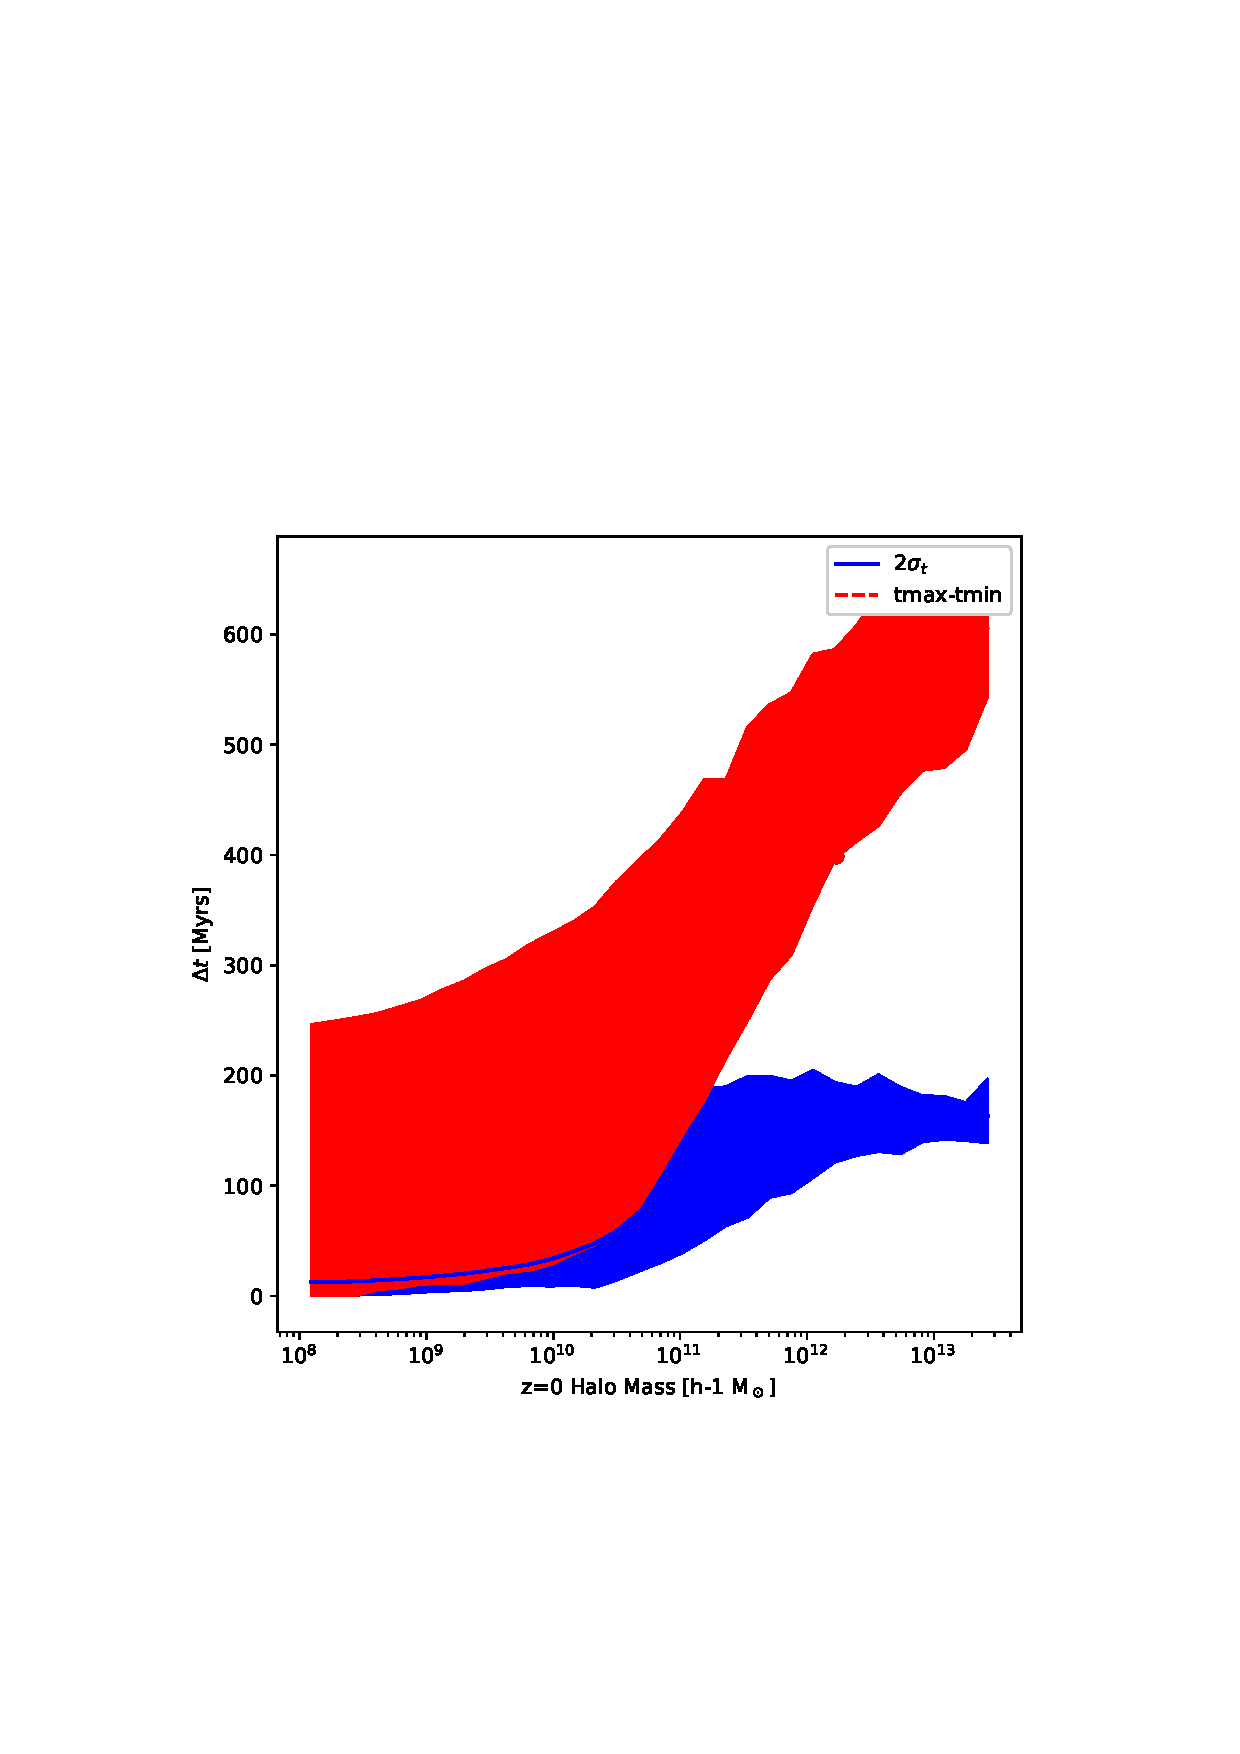
\includegraphics[width=0.94\columnwidth]{img/track_dt_2sig_LG.pdf}
\caption{\textit{Top}: The reionization time as a function of z=0 halo mass.
% : lines stand for the median value in each mass bin and shaded area cover the $5\% - 95\%$ percentiles.  
%Red stands for progenitor-based predictions while blue stands for particle-based predictions. 
The full volume reaches $x_{HI}=0.5$ at $z\sim 7.8$ (dashed line). %Reionization times correspond to a 0.5 hydrogen ionization fraction : the volume-averaged ionization fraction for the full 64 $h^{-1}$ Mpc box crosses this threshold at $t\sim 710$ Myrs ($z\sim 7.8$).
 \textit{Bottom}: The intrinsic duration of reionization  $\Delta t$ as a function of the halo mass. In both panels, lines stand for the median value within each bin of mass and  shaded area cover the $5\%-95\%$ percentiles. Dots stand for the measured values for the MW-M31 system analog.}
\label{fig:treion}
\end{figure}

The Reionization times of z=0 halos are shown in Fig. \ref{fig:treion}. Depending on the methodology used, galaxies with $M_{z=0}>10^{11} M_\odot$ reionize up to $500$ Myrs earlier than the full volume. In this mass range, the more massive the galaxies, the earlier they are reionized as expected since they host intense sources or are close to them in dense environments. At the lower masses ($M_{z=0}<10^{11} M_\odot$) the Reionization time becomes consistent with the global one.  The median time is slightly later than the global one : objects among this population are faint or even star-less and must be externally reionized. Being dense, it takes more time to reionize them than for the IGM.  Nevertheless, the scatter is quite significant from halo to halo ($\sim 250$ Myrs 5\%-95\% percentile).

The two methodologies return consistent results but with differences. The progenitor-based technique guarantees that an object is already present at high z : it returns the reionization redshift of the oldest material of a z=0 halo, thus explaining why it consistently returns lower $t_\mathrm{reion}$. On the other hand it requires that objects detectable by means of FOF pre-exist at $z>6$, biasing the sample of halos:  a $10^8 M_\odot$ halo at z=0  must have peculiar accretion rates to have a $z>6$ progenitor and still be light at z=0. The dip in reionization times at the low mass end confirms this and  by eye inspection, these objects are located in high-density regions, thus explaining their low $t_\mathrm{reion}$. It could also indicate that these objects were more massive in the past and were stripped : these low-mass objects are being assigned $t_\mathrm{reion}$ typical of more massive objects.

The particle-based methodology suffers less from this bias because all z=0 halos are considered~: the $t_\mathrm{reion}$ dip at the low-mass end disappears. However, it returns lower reionization redshifts for $M_{z=0}>10^{11} M_\odot$, resulting from  a fraction of material in halos at z=0 that was part of the diffuse matter in the IGM and was reionized at later times.

\citet{LI14} found  that $10^{12} M_\odot$ galaxies tend to reionize earlier than the IGM with $\Delta z\sim 1\pm1$ whereas we find earlier Reionization times for the same class of objects with $\Delta z\sim 1.5\pm 1.5$ (particle-based) or $\Delta z\sim 4.5\pm 3$ (progenitor-based). The differences could be related to methodologies : for instance they extrapolate reionization times using z=0 halos positions whereas we use $z>6$ progenitors or particle positions. While their approximation is appropriate for halo mass with $>10^{13} M_\odot$, we found that z=0 positions are a poor approximation of the actual halo position at high z when less massive objects are considered. Their reionization times closer to the global one could be a sign of 'signal dilution' at the lower-end of their probed range of halo mass. 
%On the other hand, our initial conditions were designed to include large clusters in a relatively small volume : it could lead to an overestimate of the UV-background 
%(as hinted by the low residual neutral fraction at z=6) 
%and an onset of the Reionization at earlier times than in their more representative large volumes. 
%The relative role played by these opposite effects is not clear yet.

%\begin{itemize}
%\item  Galaxies with $M>10^{12} M_\odot$ tend to reionize earlier than the full volume:$\sim 150-250$ myrs earlier. In this mass range, the more massive the galaxies, the earlier they are reionize as expected since they should host the most intense sources or be close to them in dense environments.
%\item At the low-mass end ($M<10^{12} M_\odot$) the reionization time becomes consistent with the global reionization time.  Note that the median time is slightly higher than the global one : it could indicate that among this population there are objects that are very faint or even without stars and must be externally reionized. Being denser, it takes more time to reionize them than in takes for the IGM.  That being said, the scatter is quite significant from to halo to halo ($\sim 120$ Myrs).
%\item Note that the two methodologies given consistent results but with slight differences. The progenitor-based technique (red curves) guarantees that an object is already formed at high z : it returns the reionization redshift of the oldest material of a z=0 halo, thus explaining why it consistently returns lower $t_\mathrm{reion}$. On the other hand since it requires that objects pre-exist at z=6, it biases the sample of halos: for instance a $10^8 M_\odot$ halo at z=0  must be quite peculiar to already have a progenitor at $z=6$ and be very light at z=0. Clearly the dip in reionization times at the low mass end confirms this. Just by eye inspections, these objects are located in high-density regions, thus explaining their lower $t_\mathrm{reion}$. It could also indicate that these objects were more massive in the past and were disrupted : these low-mass objects are being assigned $t_\mathrm{reion}$ typical of more massive objects.
%\item On the other hand, the particle-based methodology suffers less from this bias and the $t_\mathrm{reion}$ dip at the low mass end disappears. However, this method returns lower reionization redshifts and it results from the fact that a fraction, sometimes significant, of material in halos at z=0 was part of the diffuse matter and was reionized at late times. 
%\end{itemize}

\subsection{Durations of reionizations}

%\begin{figure}[ht]
%\centering 
%%\plotone{img/median_dt.pdf}
%\includegraphics[width=2.2\columnwidth]{img/median_dt.pdf}
%
%\caption{The intrinsic spread of reionization times $\Delta t$ as a function of the halo mass. The line stand for the median value within each bin of mass and the shaded area covers the $5\%-95\%$ percentiles. }
%\label{fig:dt}
%\end{figure}

Using the particles reionization times, we can investigate the intrinsic reionization duration $\Delta t$ of $t_\mathrm{reion}$ within halos : its dependance on halo mass is shown in Fig. \ref{fig:treion}. $\Delta t_{2\sigma}$ is computed from the r.m.s of particle reionization times within a halo, using $\Delta t_{2\sigma}=(\langle t_\mathrm{part}\rangle+\sigma)-(\langle t_\mathrm{part}\rangle-\sigma)$. 

$\Delta t_{2\sigma}$ increases with the halo mass with typical values of $\sim 120$ Myrs for $M_{z=0}>10^{11} M_\odot$. For $10^{12} M_\odot$, reionization durations as long as 180 Myrs or as short as 60 Myrs can be found. \citet{OCV14} made similar measurements on subhaloes of M31-MW analogs and the current results are consistent with their SPH model that shares a similar emissivity for the sources: the 120 Myrs duration found here is typical of their Reionization in isolation models, where an inside-out Reionization proceeds from the inner regions of a galaxy to its outskirts. Meanwhile the shortest $\Delta t_{2\sigma}=60$ Myrs values are typical of their external reionization scenario, where a nearby bright source 'flashes' the object. The scatter seen here would be a reflection of diverse environmental properties.

For $M>10^{11} M_\odot$, the typical values found for $\Delta t_{2\sigma}$ are comparable to the halo-to-halo scatter of $t_\mathrm{reion}$ and are likely to be lower bound values since self-shielding is not fully taken into account at our resolution. It's consistent with findings of \citet{ALV9} and \citet{LI14} for more massive objects. Consequently taking into account the variety of Reionization times to model the star formation in halos should also include the fact that within a halo the Reionization is not instantaneous. 

At low mass end, $M_{z=0}<10^{11} M_\odot$, objects have $\Delta t_{2\sigma}\sim 0$. It corresponds to the extreme case of fast external reionizations or objects small enough to fit within a single cell of the Reionization map (the $30 h^{-1}$ comoving kpc resolution corresponds to the virial radius of a $\sim 10^9 h^{-1} M_\odot$ halo). The dispersion increases toward the low mass end : as already mentioned for $t_\mathrm{reion}$ it could be due to 'stripped objects' which are being assigned $\Delta t$ typical of more massive halos. Another explanation could be tied to the small number of particles (40 for $10^8 h^{-1} M_\odot$) in such haloes, leading to greater errors in the estimate of $\sigma$.

Note that $\Delta t_{2\sigma}$ is an estimate of the duration to reionize most of the particles but time differences within a halo can be even greater.The time difference $\Delta t_\mathrm{max-min}$ between the first and the last particle to reionize is also given in Fig. \ref{fig:treion}. The most massive halos in our sample can have $\Delta t_\mathrm{max-min}=600$ Myrs and thus contain material that saw its environment reionize at very different stages.% of the Reionization.
% (as also indicated by the difference between the progenitor and particle based estimate of $t_\mathrm{reion}$). 

Lighter haloes have shorter $\Delta t_\mathrm{max-min}$ with $\Delta t_\mathrm{max-min}\sim 400$ Myrs for $10^{12} h^{-1}M_\odot$ and $\Delta t_\mathrm{max-min}< 100$ Myrs for $M<10^{10} h^{-1} M_\odot$. For this lightest class of objects, one can note that significant outliers are present, with $\Delta t_\mathrm{max-min}\sim 200$ Myrs when the median value is closer to 20 Myrs.

%\begin{itemize}
%\item Using the particle-based method, we can investigate the intrinsic spread $\Delta t$ of $t_\mathrm{reion}$ within haloes. 
%\item $\Delta t$ increases with the halo mass with typical values of $\sim 100$ Myrs for $M>10^{11} M_\odot$ (those are z=0 masses). It's comparable with the halo to halo scatter and consistant with findings of Alvarez et al. 09 and Li et al. 2014. It's important for predictions on satellite properties for instance.
%\item At low mass end we can see that some objects have $\Delta t\sim 0$ : either these objects are 'flashed' by an external field, either they are small enough to be within a single cell of the reionization map.
%\item The dispersion increases toward the low mass end : again it could be due to 'disrupted objects' which are being assigned $\Delta t$ typical of more massive haloes.
%\end{itemize}

\subsection{The case of the Local Group}

\begin{figure}[ht]
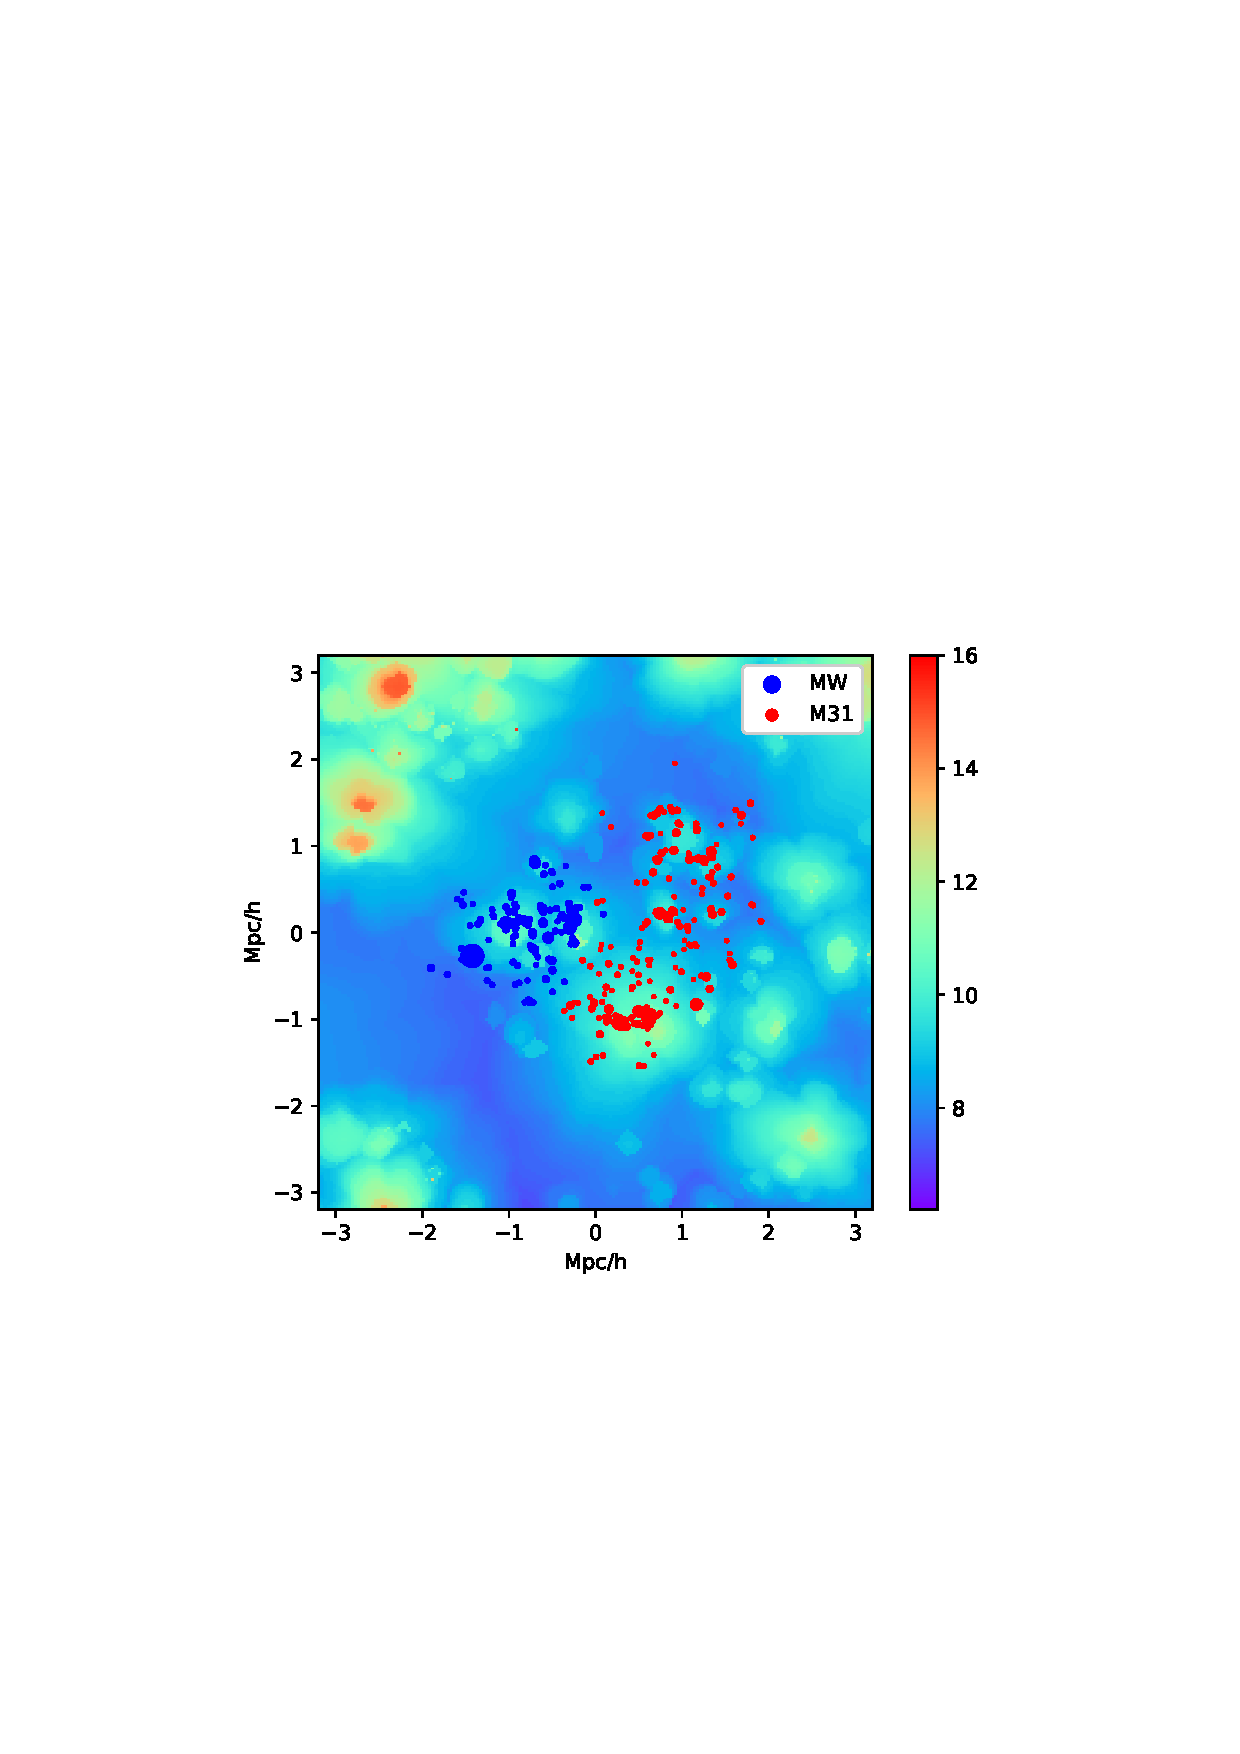
\includegraphics[width=1.2\columnwidth]{img/map_LG.png}
\caption{The EMMA reionization map around the LG (background field) and the location of GADGET halo progenitors at z=10.8 for the M31 and MW analogs (symbols). The size of the symbols are proportional to their masses. The background colors encode the reionization redshift.}
\label{fig:LG}
\end{figure}

The CLUES ICs contain an analog of the LG with two main galaxies similar to the MW ($M_{z=0}=7.7\times 10^{11} h^{-1} M_\odot$) and M31 ($M_{z=0}=1.7 \times 10^{12} h^{-1} M_\odot$) in the proper large-scale environment.

Fig. \ref{fig:LG} shows the position of their progenitors at z=10.8 within the reionization map. The MW environment reionized in a compact fashion. Meanwhile M31 reionization pattern consists in several disconnected islands, reflecting the complex and extended distribution of progenitors at these times. Both objects reionized in isolation relative to each other: the patches are easily identified and disconnected. They also reionized in isloation relative to the environment, as no reionization front seem to have swept the region.



How these two objects compare to other galaxies of similar masses ? In fig. \ref{fig:treion}, their reionization times and durations are being shown as dots, for each of the estimators. According to the progenitor-based method, M31 environment reionized earlier($z=11$) than for MW ($z=9.8$), in accordance with the measured population trend where more massive haloes tend to start their reionization earlier. Meanwhile the particle based method indicate that both objects reionized at the same time, at $z=8.2$: since these two objects are spatially close, finding that the bulk of their $z=0$ material  reionized simultaneously is not surprising. For both reionization times estimators, these two galaxies are fairly typical of their respective class of masses, albeit on the 'late reionization' side of the distribution. 

Regarding durations, $\Delta t_{2\sigma}$ are typical of the global distribution, between $100$ and $150$ Myrs. $\Delta t_{\mathrm max-min} \sim 400$ Myrs are similar for the two objects, an indication that their environments share similar extreme values for reionization times, presumably because of their closeness : it puts M31 reionization history among the most compact ones of its class of masses, maybe due to the proximity of the MW.


%\subsection{Cosmic Variance}
%\begin{figure}[ht]
%%\plotone{img/med_envir.pdf}
%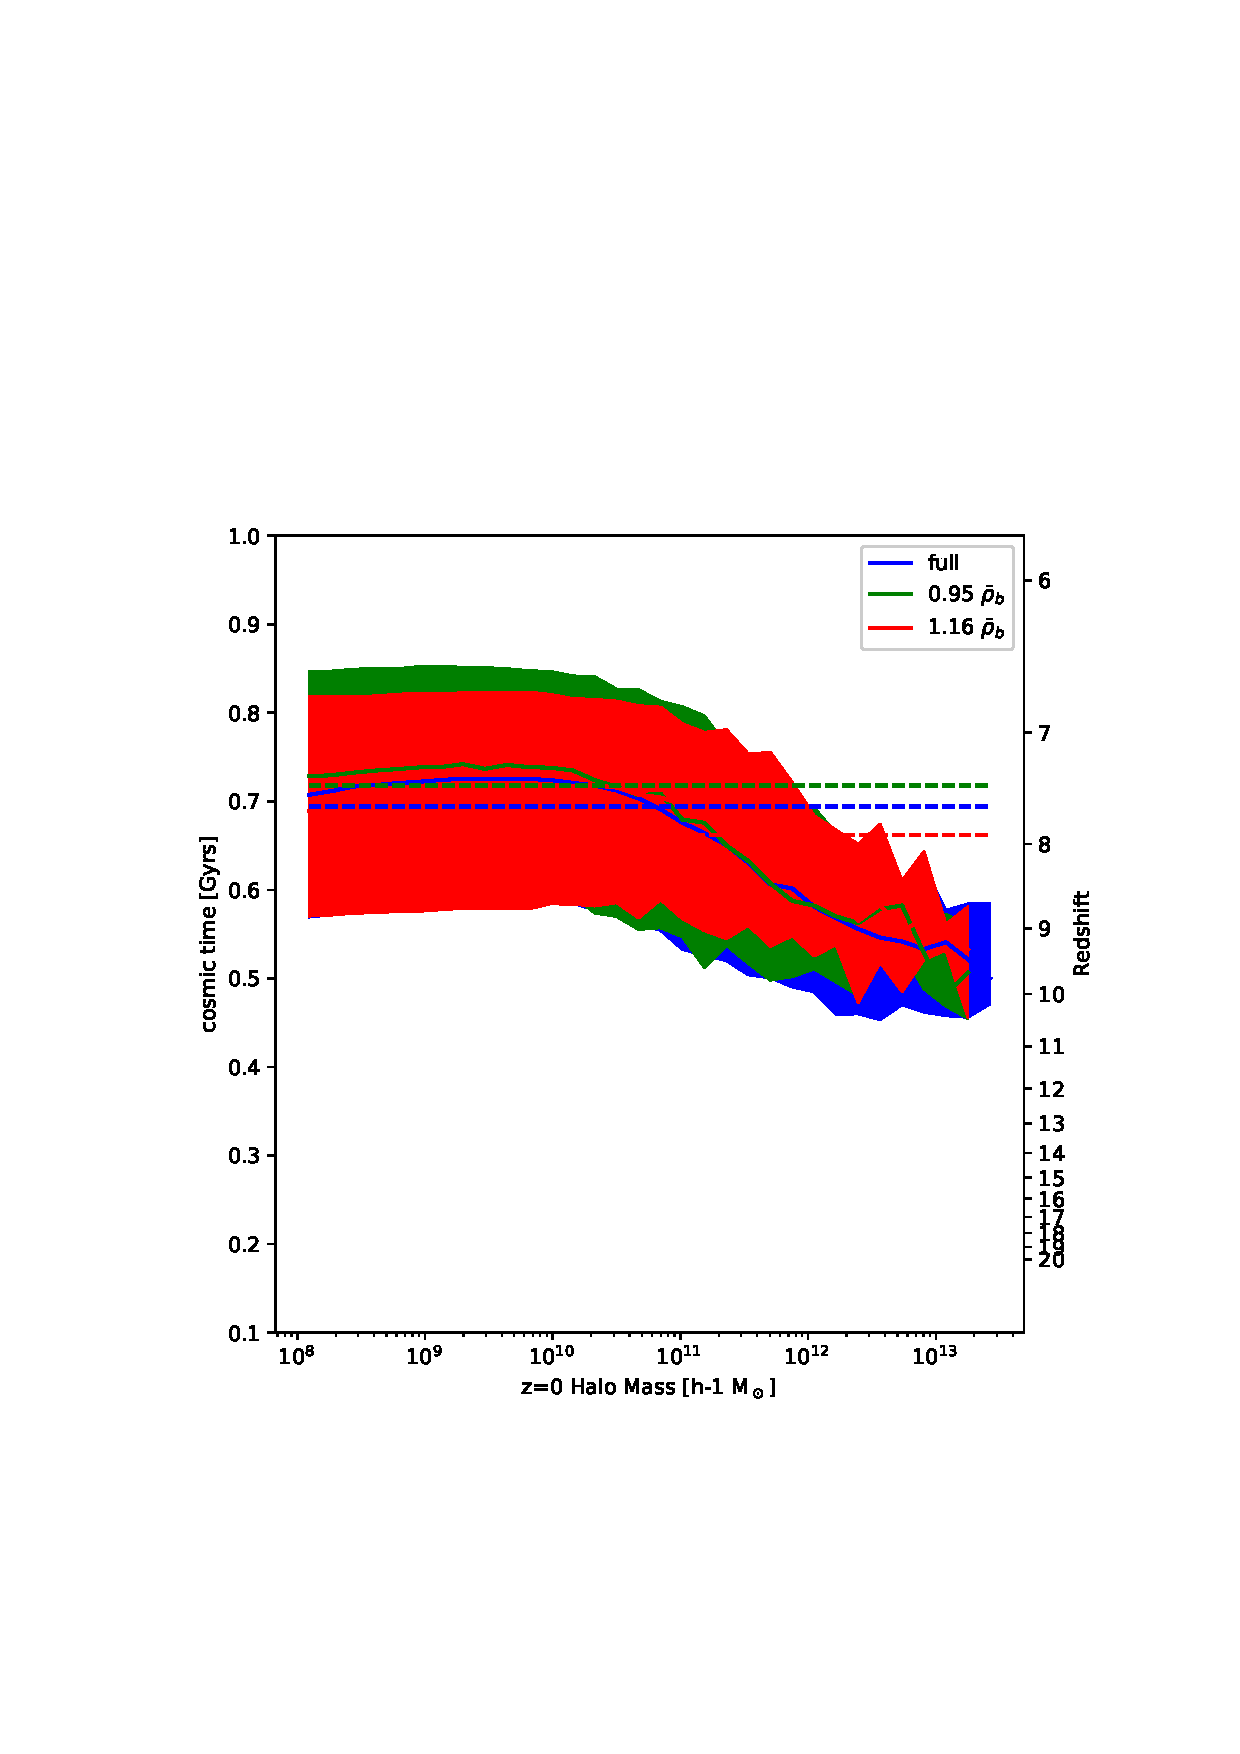
\includegraphics[height=1.10\columnwidth, width=0.94\columnwidth]{img/median_treion_envir_LG.pdf}
%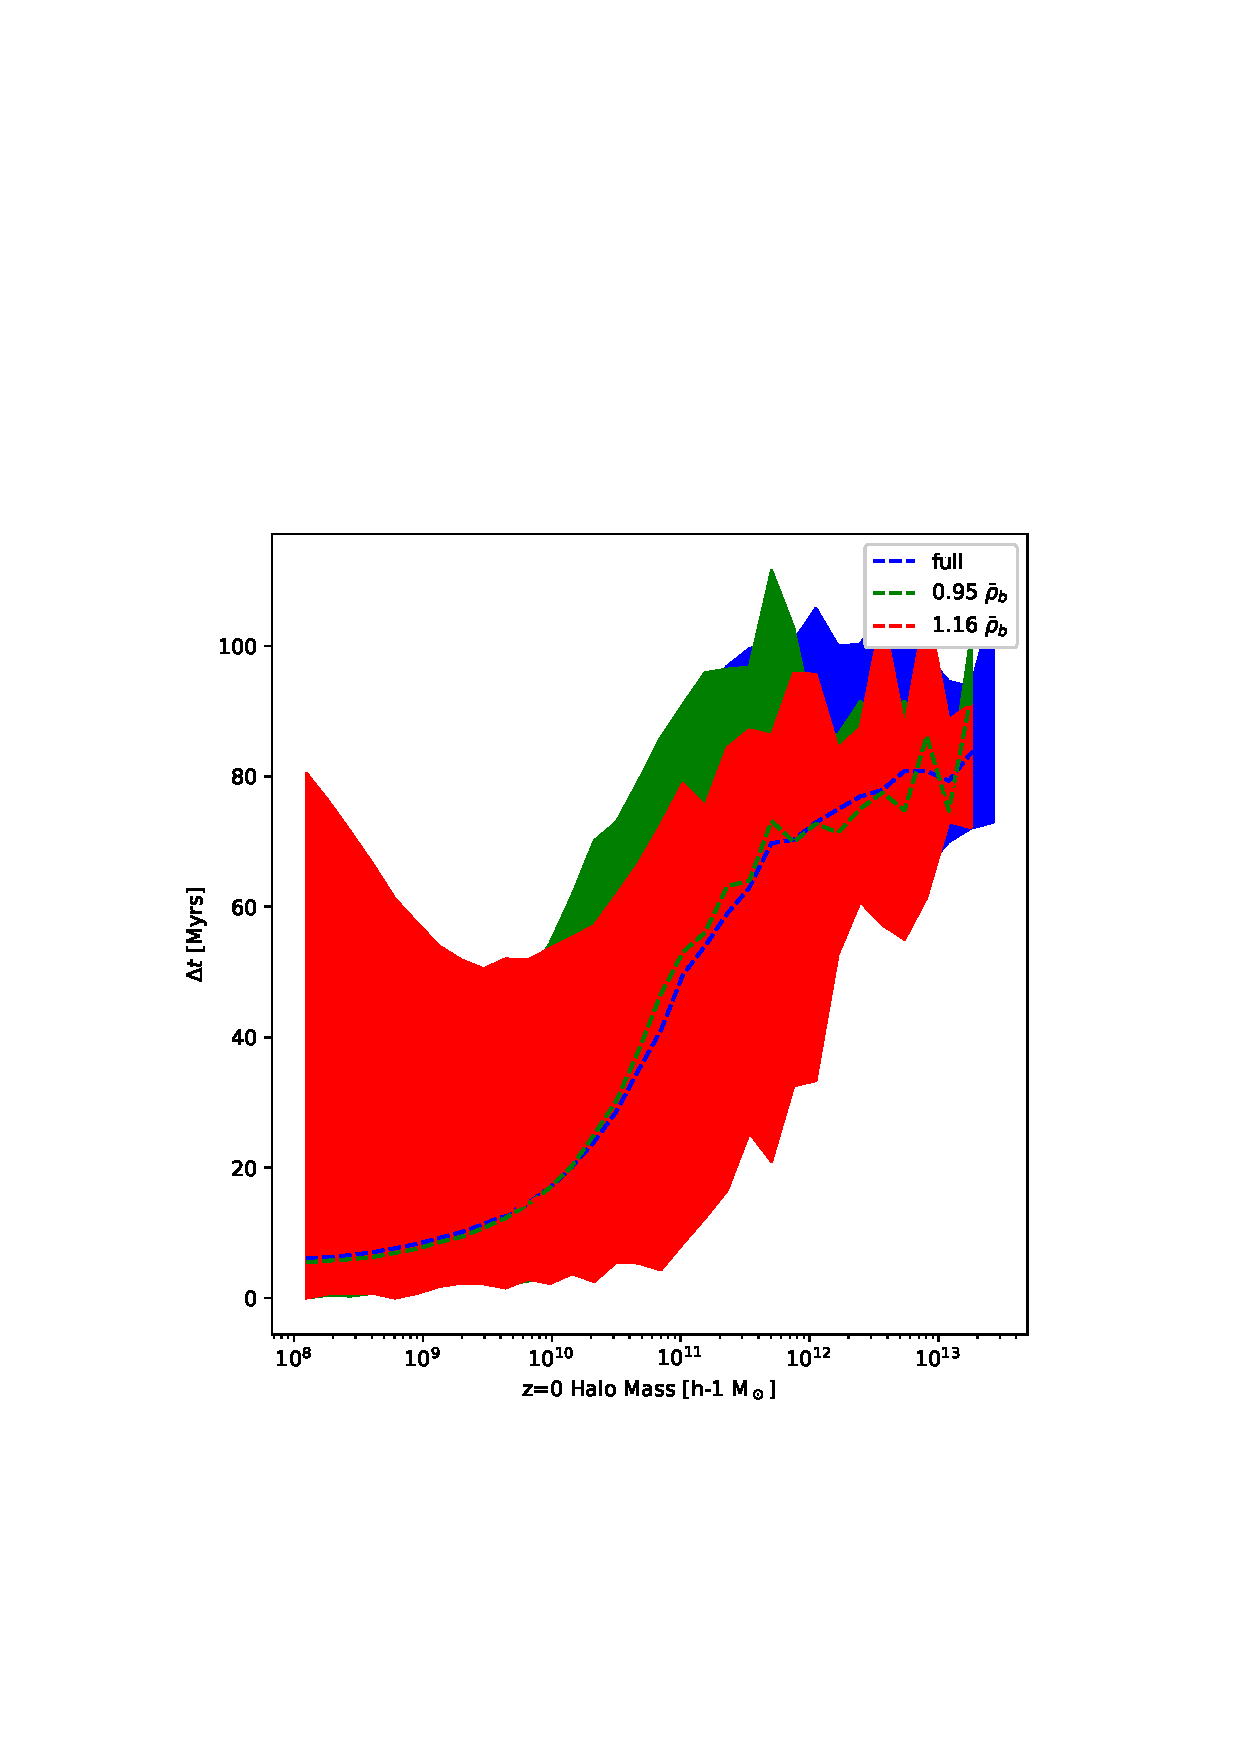
\includegraphics[width=0.94\columnwidth]{img/median_dt_envir_LG.pdf}
%\caption{Reionization times (top) and durations (bottom) as function of halo mass in two different 32$h^{-1}$ Mpc sub-volumes. Green/red stand for the most underdense/overdense octant. Blue stands for quantities computed in the full  64$h^{-1}$ Mpc volume. Lines stand for the median values in each bin of mass while the shaded area cover the $5\% - 95\%$ percentiles.  Dashed lines in the top panel stand for the reionization times of each sample.
%}
%\label{fig:envir}
%\end{figure}
%
%
% As a simple environment dependence study, we split the simulation volume in 8 identical octants. We computed the z=6 average baryon density in each of these octants and considered the most overdense (with $\rho_b\sim 1.19 \bar \rho_b$) and underdense ones (with $\rho_b\sim 0.95 \bar \rho_b$). In these octants, we recomputed the particle-based reionization times and durations (see Fig. \ref{fig:envir}). 
% 
% The scatter remains quite important, these two octants present compatibles trends and are both consistent with the one obtained from the full box. There are subtle differences nevertheless. At the low mass end, the denser the volume the lower are the reionization times as expected :  a dense volume should host bright and rare sources thus promoting an early reionization. At the high mass end however, the opposite trend can be seen : the densest octant promotes surprisingly lower reionization redshifts. It could be a small number effect which prevent convergence of these results or due to the moderation of star formation by the brightest sources in these densest environments : the most massive and brightest sources would lower the photon production of less massive objects that provide the majority of ionizing photons. The net result would be a later onset of Reionization in these regions. 
% 
% In Fig. \ref{fig:envir}, we also present the same sub-volume dependence for reionization durations $\Delta t$. Halos in the densest octant are  reionized in a more sudden manner compared to the low density sub-box and to the full volume. It's consistent with the promotion of fast external Reionizations relative to internal ones in more clustered environments. As expected, both results on $t_\mathrm{reion}$ and $\Delta t$ suggest that environment effects have a role to play.
% %, as expected. Further investigations on this role are under way.
%
%%\begin{itemize}
%%\item As a crude environment dependence study, I took advantage of the fact that the data are split in 8 identical octants. I computed the z=6 average baryon density in each of these octants and took the most overdense (with $\rho_b\sim 1.19 \bar \rho_b$) and the most underdense one (with $\rho_b\sim 0.95 \bar \rho_b$). In these two octants, I recomputed the progenitor-based reionization times
%%\item First, the scatter is quite important and at face value, these two octants present compatibles curves and are both compatibles with the one obtained from the full box.
%%\item There are subtle differences nevertheless. At the low mass end, the denser the volume the lower are the reionization times : this is the basic expectation since a dense volume should host bright and rare sources thus promoting an early reionization.
%%\item At the high mass end however, the opposite trend can be seen : the densest octant promote lower reionization redshifts. It could be a small number effect (such massive objects are rare). Or maybe this is due to the moderation of star formation by the brightest sources in these densest environments : these rare source would lower the photon production of less massive objects that provide the majority of ionizing photons ?
%%\item overall it all suggests that environment effects have a role to play, as expected, and it should be the next step.
%%\end{itemize}

%\subsection{Figure \ref{fig:dt_envir}:}
%\begin{itemize}
%\item  it's the same environment dependance study but with the intrinsic scatter $\Delta t$. We see  that halos in the densest octant are  reionized in a more sudden manner compared to the low density sub-box and to the full volume.
%\end{itemize}
 
 \section{Prospects}
%We combined for the first time the results of an AMR radiative hydrodynamics simulation of the Reionization to a z=0 DM simulation. We find that halos with $M_{z=0}$ between $10^{8}$ and $10^{13} M_\odot $ have a mass-dependent experience of the Reionization : for MW-like objects, it occurs $~150$ Myrs before the full volume with a $\sim \pm 100$ Myrs scatter. The Reionization duration within a halo can be as large as the halo-to-halo variation, implying that any modeling that includes the latter should include fluctuations of Reionization times within a galaxy for consistency. The LG reionized in isolation and within the LG, the MW and M31 ionized bubbles don't seem to overlap. Compared to the global population of galaxies, the MW and M31 experienced a slightly late and shorter reionization. 
 
%Our results complement investigations made by e.g. \citet{WEI07}, \citet{ALV9}, \citet{LI14} and \citet{OCV14}, by combining for the first time an AMR fully consistent radiative transfer simulation of the Reionization and a z=0 N-Body tree-code simulation. 

%In \citet{OCV14}, sub-haloes of M31 and MW analogs display a radial gradient of reionization redshift in their z=0 distribution : noting that our data display a similar spatial resolution, the statistics of such gradients in a population of MW-Like objects can be studied.  They would depend on the environment of halos, as implied by the wide variety of Reionization durations and by the comparisons between sub-volumes : further investigations are under way. 
%More generally, the current study underlines further that the halo mass alone is not sufficient to constrain the reionization past of an object.

%Our choices can impact our predictions. The resolution achieved here could only be obtained on moderate cosmological volumes, compared to e.g. \citet{LI14}. Such volumes are known to limit the representativity of HII regions sizes (see e.g. \citet{ILI6}) and underestimate the spatial fluctuation levels of Reionization fields. 
%Also, our initial conditions were designed to produce analogs of Local clusters~: our Reionization is therefore unlikely to be fully representative of the transition experienced by a randomly selected 64 Mpc volume . 
% The residual z=6 neutral fraction  is too low compared to Ly-$\alpha$ constraints, as also measured in the CODA I and an updated CODA II simulation (Ocvirk et al. 2014, Ocvirk et al. in prep). It could be due to an excess of radiation produced by the local overabundance of clusters, also explaining the earlier Reionization times found here for MW-like objects compared to Alvarez et al. 2009 and Li et al. 2014.

The CODA I-AMR simulation and its combination to a CLUES DM simulation are the results of a long-term development strategy and  challenging productions runs. Taken in conjunction with previous works, we believe that our results establish further the picture of an early, diverse and not instantaneous Reionization as seen by galaxies. 

The models can  be improved. For example, the inclusion of AGNs would lead to another sources of environmental fluctuations (see e.g. \citet{CHA15}), whereas models for star formation driven e.g. by molecular or metal cooling (see e.g. \citet{WIS9}) could modify the distribution of photons production among the halo classes. Likewise the volumes probed here are known to limit the representativity of HII regions sizes (see e.g. \citet{ILI6}) and underestimate the spatial fluctuation levels of Reionization fields. These effects can modify our quantitative predictions, but we don't expect them to alter substantially our predictions, notably on the LG members.

Future investigations will include the environmental dependence of our results, as we expect field galaxies to experience the Reionization differently than members of groups or clusters. We also aim at investigating the detailed structure of the Reionization within haloes, notably in relation to their substructures. A special focus will be put on the LG members and how to translate our predictions into observable quantites to be compared to the local population of satellite galaxies. Hopefully, this letter will act as the building block for these forthcoming studies based on the CODA~I-AMR run.


%On the other hand, this work %in conjunction to previous ones 
%establishes further the diverse view of the Reionization as seen by galaxies~: 


%\begin{itemize}
%\item Limitations of the model : resolution, volume limitations, no AGN, H2, metals,etc..
%\item How does it compares to Alvarez et al. 09 and Li et al. 2014 (Method) ? The current volume is much smaller and our resolution is much higher than these previous studies : as a consequence the range of halo mass probed here is much more consistent with galactic scales. We use actual coupled radiative hydrodynamics simulation instead of semi-numerical models. We use z=6 positions to assign Reionization redshifts instead of z=0 ones, which I think is much more representative of the actual Reionization history : note that since we are investigating halos with lower masses, their peculiar motion is likely higher and using their z=0 positions is likely to be a very poor approximation of their location at high-z. In fact, that's how it has been done at first and the trends are almost completely washed out. 
%\item How does it compares to Alvarez et al. 09 and Li et al. 2014 (Results) ? They are consistent with a slight tendency to have higher Reionization redshifts in our case in the range of mass that overlaps : typically they find a $\Delta z\sim 1 \pm 1$ for $M\sim10^{12} M_\odot$ while here we have $\Delta z\sim 2.5 \pm 2$. It could be explained by different methodologies (z=0 vs z=6 position for instance) or population statistics (their boxes are larger but less resolved). In terms of intrinsic scatter $\Delta t$, the results are fully consistent but the scatter are quite large, both in ours and theirs studies.
%\end{itemize}

 
 

\acknowledgments
ANR ORAGE, ANR EMMA, INCITE Project, ORNL Staff, etc...
XXXXXXXX XXXXXXXX XXXXXXXX XXXXXXXX XXXXXXXX XXXXXXXX XXXXXXXX XXXXXXXX XXXXXXXX XXXXXXXX XXXXXXXXXXXXXXXX XXXXXXXXXXXXXXXXXXXXXXXX XXXXXXXX XXXXXXXX XXXXXXXXXXXXXXXX 

%\appendix

%\begin{thebibliography}{}
%\bibitem[{{Alvarez} {et~al.}(2009){Alvarez}, {Busha}, {Abel}, \&
%  {Wechsler}}]{ALV9}
%{Alvarez}, M.~A., {Busha}, M., {Abel}, T., \& {Wechsler}, R.~H. 2009, \apjl,
%  703, L167
%
%\bibitem[{{Aubert} {et~al.}(2015){Aubert}, {Deparis}, \& {Ocvirk}}]{AUB15}
%{Aubert}, D., {Deparis}, N., \& {Ocvirk}, P. 2015, \mnras, 454, 1012
%
%\bibitem[{{Bouwens} {et~al.}(2014){Bouwens}, {Bradley}, \&
%  {Seitz}}]{BOU14}
%{Bouwens}, R.~J., {Bradley}, L., {Zitrin}, A., {et~al.} 2014, \apj, 795, 126
%
%\bibitem[{{Brown} {et~al.}(2014){Brown}, {Tumlinson} \& {Renzini}}]{BROWN14}
%{Brown}, T.~M., {Tumlinson}, J., {Geha}, M., {et~al.} 2014, \apj, 796, 91
%
%\bibitem[{{Busha} {et~al.}(2010){Busha}, {Alvarez}, {Wechsler}, {Abel}, \&
%  {Strigari}}]{BUS10}
%{Busha}, M.~T., {Alvarez}, M.~A., {Wechsler}, R.~H., {Abel}, T., \& {Strigari},
%  L.~E. 2010, \apj, 710, 408
%
%\bibitem[{{Chardin} {et~al.}(2015){Chardin}, {Haehnelt}, {Aubert}, \&
%  {Puchwein}}]{CHA15}
%{Chardin}, J., {Haehnelt}, M.~G., {Aubert}, D., \& {Puchwein}, E. 2015, \mnras,
%  453, 2943
%
%\bibitem[{{Deparis} {et~al.}(2017){Deparis}, {Aubert}, {Ocvirk}, \&
%  {Gillet}}]{DEP17}
%{Deparis}, N., {Aubert}, D., {Ocvirk}, P., \& {Gillet}, N. 2017, in prep.,
%  arXiv:1005.2687
%
%\bibitem[{Fan {et~al.}(2006)Fan, Carilli, \& Keating}]{FAN6}
%Fan, X., Carilli, C.~L., \& Keating, B. 2006,\araa, 44, 415.
%%\newblock \url{http://adsabs.harvard.edu/abs/2006ARA%26A..44..415F}
%
%\bibitem[{{Finkelstein} {et~al.}(2015){Finkelstein}, {Ryan}, \& {Willner}}]{FIN15}
%{Finkelstein}, S.~L., {Ryan}, Jr., R.~E., {Papovich}, C., {et~al.} 2015, \apj,
%  810, 71
%
%\bibitem[{{Gillet} {et~al.}(2015){Gillet}, {Ocvirk}, {Aubert} \& {Hoffman}}]{GIL15}
%{Gillet}, N., {Ocvirk}, P., {Aubert}, D., {et~al.} 2015, \apj, 800, 34
%
%\bibitem[{{Gottloeber} {et~al.}(2010){Gottloeber}, {Hoffman}, \&
%  {Yepes}}]{GOT10}
%{Gottloeber}, S., {Hoffman}, Y., \& {Yepes}, G. 2010, ArXiv e-prints,
%  arXiv:1005.2687
%
%\bibitem[{{Hinshaw} {et~al.}(2009){Hinshaw}, {Weiland}\& {Wright}}]{HIN9}
%{Hinshaw}, G., {Weiland}, J.~L., {Hill}, R.~S., {et~al.} 2009, \apjs, 180, 225
%
%\bibitem[{{Iliev} {et~al.}(2006){Iliev}, {Mellema}, {Pen}, {Merz}, {Shapiro},
%  \& {Alvarez}}]{ILI6}
%{Iliev}, I.~T., {Mellema}, G., {Pen}, U.-L., {et~al.} 2006, \mnras, 369, 1625
%
%\bibitem[{{Iliev} {et~al.}(2011){Iliev}, {Moore}, {Gottl{\"o}ber}, {Yepes},
%  {Hoffman}, \& {Mellema}}]{ILI11}
%{Iliev}, I.~T., {Moore}, B., {Gottl{\"o}ber}, S., {et~al.} 2011, \mnras, 413,
%  2093
%
%\bibitem[{{Koposov} {et~al.}(2009){Koposov}, {Yoo}, {Rix}, {Weinberg},
%  {Macci{\`o}}, \& {Escud{\'e}}}]{KOP9}
%{Koposov}, S.~E., {Yoo}, J., {Rix}, H.-W., {et~al.} 2009, \apj, 696, 2179
%
%\bibitem[{Leitherer {et~al.}(1999)Leitherer, Schaerer, Goldader, Delgado,
%  Robert, Kune, de~Mello, Devost, \& Heckman}]{LEI99}
%Leitherer, C., Schaerer, D., Goldader, J.~D., {et~al.} 1999, \apjs, 123, 3.
%%\newblock \url{http://adsabs.harvard.edu/abs/1999ApJS..123....3L}
%
%\bibitem[{{Li} {et~al.}(2014){Li}, {Alvarez}, {Wechsler}, \& {Abel}}]{LI14}
%{Li}, T.~Y., {Alvarez}, M.~A., {Wechsler}, R.~H., \& {Abel}, T. 2014, \apj,
%  785, 134
%
%\bibitem[{{Ocvirk} \& {Aubert}(2011)}]{OCV11}
%{Ocvirk}, P., \& {Aubert}, D. 2011, \mnras, 417, L93
%
%\bibitem[{{Ocvirk} {et~al.}(2014){Ocvirk}, {Gillet}, {Aubert} \& {Hoffman}}]{OCV14}
%{Ocvirk}, P., {Gillet}, N., {Aubert}, D., {et~al.} 2014, \apj, 794, 20
%
%\bibitem[{{Ocvirk} {et~al.}(2016){Ocvirk}, {Gillet}\& {Stranex}}]{OCV16}
%{Ocvirk}, P., {Gillet}, N., {Shapiro}, P.~R., {et~al.} 2016, \mnras, 463, 1462
%
%\bibitem[{{Planck Collaboration} {et~al.}(2015){Planck Collaboration}, Ade,
%  Aghanim}]{PLA15}
%{Planck Collaboration}, Ade, P. A.~R., Aghanim, N., {et~al.} 2015, ArXiv
%  e-prints, 1502, arXiv:1502.01589.
%%\newblock \url{http://adsabs.harvard.edu/abs/2015arXiv150201589P}
%
%
%%\bibitem[{{Planck Collaboration} {et~al.}(2015){Planck Collaboration}, Ade,
%%  Aghanim, Arnaud, Ashdown, Aumont, Baccigalupi, Banday, Barreiro, Bartlett,
%%  Bartolo, Battaner, Battye, Benabed, Benoit, Benoit-Levy, Bernard, Bersanelli,
%%  Bielewicz, Bonaldi, Bonavera, Bond, Borrill, Bouchet, Boulanger, Bucher,
%%  Burigana, Butler, Calabrese, Cardoso, Catalano, Challinor, Chamballu, Chary,
%%  Chiang, Chluba, Christensen, Church, Clements, Colombi, Colombo, Combet,
%%  Coulais, Crill, Curto, Cuttaia, Danese, Davies, Davis, de~Bernardis, de~Rosa,
%%  de~Zotti, Delabrouille, Desert, Di~Valentino, Dickinson, Diego, Dolag, Dole,
%%  Donzelli, Dore, Douspis, Ducout, Dunkley, Dupac, Efstathiou, Elsner, Ensslin,
%%  Eriksen, Farhang, Fergusson, Finelli, Forni, Frailis, Fraisse, Franceschi,
%%  Frejsel, Galeotta, Galli, Ganga, Gauthier, Gerbino, Ghosh, Giard,
%%  Giraud-Heraud, Giusarma, Gjerlow, Gonzalez-Nuevo, Gorski, Gratton, Gregorio,
%%  Gruppuso, Gudmundsson, Hamann, Hansen, Hanson, Harrison, Helou,
%%  Henrot-Versille, Hernandez-Monteagudo, Herranz, Hildebrandt, Hivon, Hobson,
%%  Holmes, Hornstrup, Hovest, Huang, Huffenberger, Hurier, Jaffe, Jaffe, Jones,
%%  Juvela, Keihanen, Keskitalo, Kisner, Kneissl, Knoche, Knox, Kunz,
%%  Kurki-Suonio, Lagache, Lahteenmaki, Lamarre, Lasenby, Lattanzi, Lawrence,
%%  Leahy, Leonardi, Lesgourgues, Levrier, Lewis, Liguori, Lilje, Linden-Vornle,
%%  Lopez-Caniego, Lubin, Macias-Perez, Maggio, Maino, Mandolesi, Mangilli,
%%  Marchini, Martin, Martinelli, Martinez-Gonzalez, Masi, Matarrese, Mazzotta,
%%  McGehee, Meinhold, Melchiorri, Melin, Mendes, Mennella, Migliaccio, Millea,
%%  Mitra, Miville-Deschenes, Moneti, Montier, Morgante, Mortlock, Moss, Munshi,
%%  Murphy, Naselsky, Nati, Natoli, Netterfield, Norgaard-Nielsen, Noviello,
%%  Novikov, Novikov, Oxborrow, Paci, Pagano, Pajot, Paladini, Paoletti,
%%  Partridge, Pasian, Patanchon, Pearson, Perdereau, Perotto, Perrotta,
%%  Pettorino, Piacentini, Piat, Pierpaoli, Pietrobon, Plaszczynski,
%%  Pointecouteau, Polenta, Popa, Pratt, Prezeau, Prunet, Puget, Rachen, Reach,
%%  Rebolo, Reinecke, Remazeilles, Renault, Renzi, Ristorcelli, Rocha, Rosset,
%%  Rossetti, Roudier, Rouille~d'Orfeuil, Rowan-Robinson, Rubino-Martin,
%%  Rusholme, Said, Salvatelli, Salvati, Sandri, Santos, Savelainen, Savini,
%%  Scott, Seiffert, Serra, Shellard, Spencer, Spinelli, Stolyarov, Stompor,
%%  Sudiwala, Sunyaev, Sutton, Suur-Uski, Sygnet, Tauber, Terenzi, Toffolatti,
%%  Tomasi, Tristram, Trombetti, Tucci, Tuovinen, Turler, Umana, Valenziano,
%%  Valiviita, Van~Tent, Vielva, Villa, Wade, Wandelt, Wehus, White, White,
%%  Wilkinson, Yvon, Zacchei, \& Zonca}]{PLA15}
%%{Planck Collaboration}, Ade, P. A.~R., Aghanim, N., {et~al.} 2015, ArXiv
%%  e-prints, 1502, arXiv:1502.01589.
%%\newblock \url{http://adsabs.harvard.edu/abs/2015arXiv150201589P}
%
%\bibitem[{{Springel}(2005)}]{SPR5}
%{Springel}, V. 2005, \mnras, 364, 1105
%
%\bibitem[{{Wise} \& {Cen}(2009)}]{WIS9}
%{Wise}, J.~H., \& {Cen}, R. 2009, \apj, 693, 984
%
%\end{thebibliography}

%\bibliographystyle{aasjournal}
%\bibliography{sample61}

\begin{thebibliography}{}

\bibitem[Alvarez et al.(2009)]{ALV9} Alvarez, M.~A., Busha, M., Abel, T., \& Wechsler, R.~H. 2009, \apjl,
  703, L167
\bibitem[Aubert et al.(2015)]{AUB15} Aubert, D., Deparis, N., \& Ocvirk, P. 2015, \mnras, 454, 1012
\bibitem[{Bouwens} {et~al.}(2014)]{BOU14} {Bouwens}, R.~J., {Bradley}, L., {Zitrin}, A., {et~al.} 2014, \apj, 795, 126
\bibitem[{Brown} {et~al.}(2014)]{BROWN14} {Brown}, T.~M., {Tumlinson}, J., {Geha}, M., {et~al.} 2014, \apj, 796, 91
\bibitem[{{Busha} {et~al.}(2010)}]{BUS10} {Busha}, M.~T., {Alvarez}, M.~A., {Wechsler}, R.~H., {Abel}, T., \& {Strigari}, L.~E. 2010, \apj, 710, 408
\bibitem[{{Chardin} {et~al.}(2015)}]{CHA15} {Chardin}, J., {Haehnelt}, M.~G., {Aubert}, D., \& {Puchwein}, E. 2015, \mnras, 453, 2943
\bibitem[{{D'Aloiso} {et~al.}(2015)}]{ALO15}{D'Aloisio}, A., {McQuinn}, M., {Trac}, H. 2015,\apjl, 813, L38
\bibitem[{{Davies \& Furlanetto}(2016)}]{DAV16} {Davies}, F.~B. and {Furlanetto}, S.~R.,\mnras, 460, 1328
\bibitem[{{Deparis} {et~al.}(2017)}]{DEP17}{Deparis}, N., {Aubert}, D., {Ocvirk}, P., \& {Gillet}, N. 2017, in prep.,
  arXiv:1005.2687
\bibitem[{{Dixon} {et~al.}(2017)}]{DIX17}{Dixon}, K.,{Iliev}, I.,{Gottl{\"o}ber}, S.
	{Yepes}, G. ,{et~al.} 2017,arXiv:1703.06140
\bibitem[{Fan {et~al.}(2006)}]{FAN6} Fan, X., Carilli, C.~L., \& Keating, B. 2006, \araa, 44, 415.
\bibitem[{{Finkelstein} {et~al.}(2015)}]{FIN15}{Finkelstein}, S.~L., {Ryan}, Jr., R.~E., {Papovich}, C., {et~al.} 2015, \apj, 810, 71
\bibitem[{{Gillet} {et~al.}(2015)}]{GIL15} {Gillet}, N., {Ocvirk}, P., {Aubert}, D., {et~al.} 2015, \apj, 800, 34
\bibitem[{{Gottloeber} {et~al.}(2010)}]{GOT10} {Gottloeber}, S., {Hoffman}, Y., \& {Yepes}, G. 2010, ArXiv e-prints, arXiv:1005.2687
\bibitem[{{Hinshaw} {et~al.}(2009)}]{HIN9} {Hinshaw}, G., {Weiland}, J.~L., {Hill}, R.~S., {et~al.} 2009, \apjs, 180,225
\bibitem[{{Iliev} {et~al.}(2006)}]{ILI6}{Iliev}, I.~T., {Mellema}, G., {Pen}, U.-L., {et~al.} 2006, \mnras, 369, 1625
\bibitem[{{Iliev} {et~al.}(2011)}]{ILI11}{Iliev}, I.~T., {Moore}, B., {Gottl{\"o}ber}, S., {et~al.} 2011, \mnras, 413,
  2093
\bibitem[{{Koposov} {et~al.}(2009)}]{KOP9} {Koposov}, S.~E., {Yoo}, J., {Rix}, H.-W., {et~al.} 2009, \apj, 696, 2179
\bibitem[{Leitherer {et~al.}(1999)}]{LEI99} Leitherer, C., Schaerer, D., Goldader, J.~D., {et~al.} 1999, \apjs, 123, 3.
\bibitem[{{Li} {et~al.}(2014)}]{LI14} {Li}, T.~Y., {Alvarez}, M.~A., {Wechsler}, R.~H., \& {Abel}, T. 2014, \apj, 785, 134
\bibitem[{{Ocvirk} \& {Aubert}(2011)}]{OCV11}{Ocvirk}, P., \& {Aubert}, D. 2011, \mnras, 417, L93
\bibitem[{{Ocvirk} {et~al.}(2014)}]{OCV14}{Ocvirk}, P., {Gillet}, N., {Aubert}, D., {et~al.} 2014, \apj, 794, 20
\bibitem[{{Ocvirk} {et~al.}(2016)}]{OCV16} {Ocvirk}, P., {Gillet}, N., {Shapiro}, P.~R., {et~al.} 2016, \mnras, 463, 1462
\bibitem[{{Planck Collaboration} {et~al.}(2015)}]{PLA15} {Planck Collaboration}, Ade, P. A.~R., Aghanim, N., {et~al.} 2015, ArXiv e-prints, 1502, arXiv:1502.01589.
\bibitem[{{Springel}(2005)}]{SPR5} {Springel}, V. 2005, \mnras, 364, 1105
\bibitem[{{Weinmann} {et~al.}(2007)}]{WEI07} {Weinmann}, S., {Maccio}, A., {Iliev}, I., {et~al.} 2007, \mnras, 381,367
\bibitem[{{Wise} \& {Cen}(2009)}]{WIS9} {Wise}, J.~H., \& {Cen}, R. 2009, \apj, 693, 984

%\bibitem[Astropy Collaboration et al.(2013)]{2013A&A...558A..33A} Astropy Collaboration, Robitaille, T.~P., Tollerud, E.~J., et al.\ 2013, \aap, 558, A33 
%\bibitem[Bertin \& Arnouts(1996)]{1996A&AS..117..393B} Bertin, E., \& Arnouts, S.\ 1996, \aaps, 117, 393 
%\bibitem[Corrales(2015)]{2015ApJ...805...23C} Corrales, L.\ 2015, \apj, 805, 23
%\bibitem[Ferland et al.(2013)]{2013RMxAA..49..137F} Ferland, G.~J., Porter, R.~L., van Hoof, P.~A.~M., et al.\ 2013, \rmxaa, 49, 137
%\bibitem[Hanisch \& Biemesderfer(1989)]{1989BAAS...21..780H} Hanisch, R.~J., \& Biemesderfer, C.~D.\ 1989, \baas, 21, 780 
%\bibitem[Lamport(1994)]{lamport94} Lamport, L. 1994, LaTeX: A Document Preparation System, 2nd Edition (Boston, Addison-Wesley Professional)
%\bibitem[Schwarz et al.(2011)]{2011ApJS..197...31S} Schwarz, G.~J., Ness, J.-U., Osborne, J.~P., et al.\ 2011, \apjs, 197, 31  
%\bibitem[Vogt et al.(2014)]{2014ApJ...793..127V} Vogt, F.~P.~A., Dopita, M.~A., Kewley, L.~J., et al.\ 2014, \apj, 793, 127  

\end{thebibliography}

%% This command is needed to show the entire author+affilation list when
%% the collaboration and author truncation commands are used.  It has to
%% go at the end of the manuscript.
%\allauthors

%% Include this line if you are using the \added, \replaced, \deleted
%% commands to see a summary list of all changes at the end of the article.
%\listofchanges

\end{document}

% End of file `sample61.tex'.
